The development set selected constant action 3: a 120-m proposal step and price 0.0125. Against that setting, the mean of the three short PPO policies changes mean interval reward by -0.00607 [-0.00743, -0.00449], post-warmup coverage by -0.87 [-1.03, -0.69] percentage points and energy by -44.84 [-48.44, -41.46] Wh. These intervals resample eight mission-seed blocks while keeping the three learned policies fixed; they do not quantify performance across the population of possible training runs.
\begin{table}[t]\centering\small
\caption{Held-out short-PPO evaluation: 32 missions per policy, after 2048 steps per training seed.}
\begin{tabular}{lrrr}\toprule Policy & Mean reward & $\bar C$ & $E$ [Wh]\\\midrule
constant 3 & 0.6259 & 0.6348 & 329.2 \\
constant 4 & 0.6255 & 0.6331 & 310.4 \\
ppo seed0 & 0.6168 & 0.6217 & 261.9 \\
ppo seed1 & 0.6259 & 0.6348 & 329.2 \\
ppo seed2 & 0.6168 & 0.6217 & 261.9 \\
\bottomrule\end{tabular}\label{tab:v4rl}\end{table}
\begin{figure*}[tbp]\centering
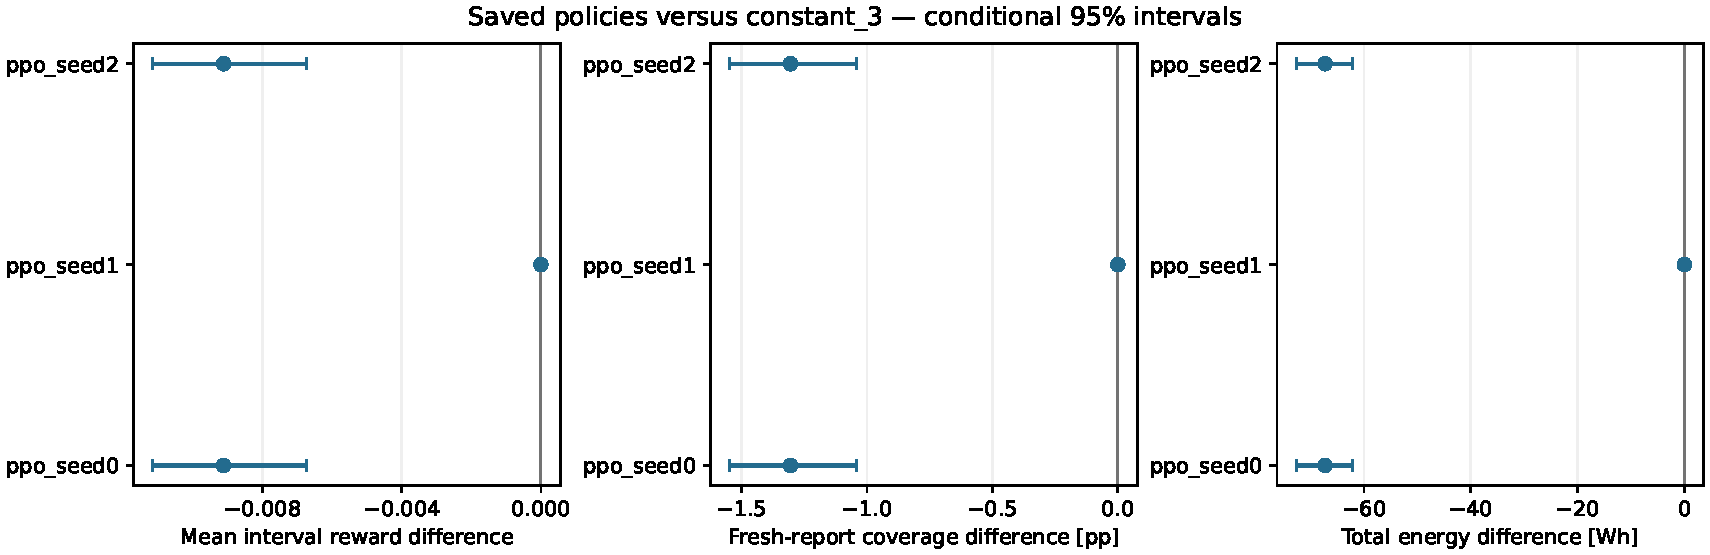
\includegraphics[width=.98\textwidth]{figures/ppo_v4.pdf}
\caption{Each short PPO training seed compared with the development-selected constant setting on the same held-out world seeds. Intervals condition on the trained policies. Favorable energy differences are negative; favorable reward and coverage differences are positive.}
\label{fig:v4ppo}\end{figure*}
The three training runs completed at 2.74--3.70 steps/s on a shared CPU. A separate 256-step, two-chunk run exercised the progress wrapper and optimizer continuation. Neither that software check nor a 2048-step pilot establishes convergence. The useful deliverable is a reproducible way to test learning against strong fixed settings, with no guarantee that extra training improves coverage or reward.
Action logs show that ppo seed0 used action 1 at every evaluated decision; ppo seed1 used action 3 at every evaluated decision; ppo seed2 used action 1 at every evaluated decision. This observed constant behavior provides no evidence of learned state-dependent adaptation, even when its score matches a strong fixed setting.
